\chapter{Machine Learning and Cybersecurity}\label{ch:machine-learning-and-cybersecurity}

\begin{figure}[htb]
    \centering
    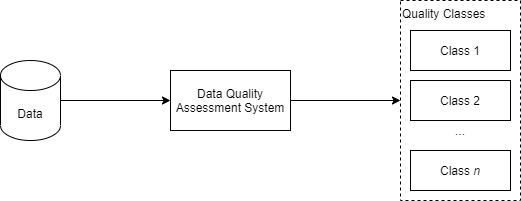
\includegraphics[width=0.9\textwidth]{figures/dq-simple.png}
    \caption{}
    \label{fig:dq-simple}
\end{figure}
\FloatBarrier

\begin{figure}[htb]
    \centering
    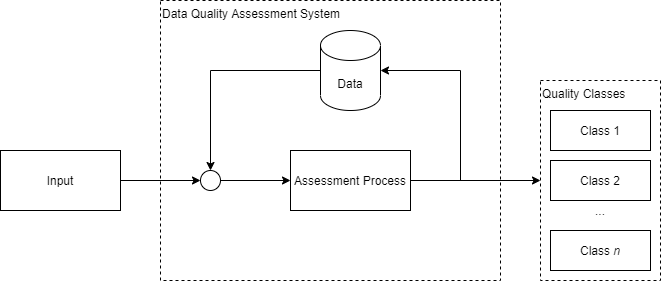
\includegraphics[width=0.9\textwidth]{figures/dq-system.png}
    \caption{}
    \label{fig:dq-system}
\end{figure}
\FloatBarrier

\section{Data Quality Attributes}

Eppler (2006) presented list of seventy of the most used data and information quality criteria explicitly defined in the literature.
They provide criterial basis for most of the DQ frameworks.
The list is shown in the figure~\ref{fig:dq-criteria}.

\begin{figure}[htb]
    \begin{multicols}{3}
        \begin{enumerate}
            \item Comprehensiveness
            \item Accuracy
            \item Clarity
            \item Applicability
            \item Conciseness
            \item Consistency
            \item Correctness
            \item Currency
            \item Convenience
            \item Timeliness
            \item Traceability
            \item Interactivity
            \item Accessibility
            \item Security
            \item Maintainability
            \item Speed
            \item Objectivity
            \item Attributability
            \item Value-added
            \item Reputation (source)
            \item Ease-of-use
            \item Precision
            \item Comprehensibility
            \item Trustworthiness\newline (source)
            \item Reliability
            \item Price 
            \item Verifiability
            \item Testability
            \item Provability
            \item Performance
            \item Ethics
            \item Privacy
            \item Helpfulness
            \item Neutrality
            \item Ease of Manipulation
            \item Validity
            \item Relevance
            \item Coherence
            \item Interpretability
            \item Completeness
            \item Learnability
            \item Exclusivity
            \item Right Amount
            \item Existence of meta information
            \item Appropriateness\newline of meta information
            \item Target group orientation
            \item Reduction of complexity
            \item Response time
            \item Believability
            \item Availability
            \item Consistent Representation
            \item Ability to represent null values
            \item Semantic Consistency
            \item Concise Representation
            \item Obtainability
            \item Stimulating
            \item Attribute granularity
            \item Flexibility
            \item Reflexivity
            \item Robustness
            \item Equivalence of redundant or distributed data
            \item Concurrency of redundant or distributed data
            \item Nonduplication
            \item Essentialness
            \item Rightness
            \item Usability
            \item Cost
            \item Ordering
            \item Browsing
            \item Error rate
        \end{enumerate}
    \end{multicols}

    \centering
    \caption{Data \& Information Quality Criteria~\cite{eppler2006}}
    \label{fig:dq-criteria}
\end{figure}
\FloatBarrier

Uniqueness
Accuracy
Consistency
Completeness
Timeliness
Currency
Format Compliance
Referential Integrity

% \section{AI as a~tool for security breaches mitigation}\label{sec:ai-as-a-tool-for-security-breaches-mitigation}

%In the section~\ref{subsec:evasion} the principle of \textbf{model verifiability} was already mentioned.

\subsection{Parallel hybrid systems}\label{subsec:parallel-hybrid-systems}

In the paper \say{Is machine learning cybersecurity's silver bullet?} ESET's experts sort training data into three groups - malicious, clean and potentially unwanted.
They recommend not to use algorithm own output data as inputs, because any further errors are reinforced and multiplied, as the same incorrect result enters a~loop and creates more false positives or misses of malicious items.
In the next chapter ESET points out how crucial it is to achieve an equilibrium of sufficient protection from malicious items and false positives minimised to a~manageable level.
Finally, in the chapter \textit{Machine learning by ESET - The road to augur} authors let us take a~look under the hood of their ML engine called Augur.
For malicious file detection they are using two branches:
\begin{enumerate*}[label=(\roman*)]
    \item sandbox analysis followed by advanced memory analysis and behavioural features extraction (these features are later used to train ML models),
    \item ML-based branch.
\end{enumerate*}
ML-based branch consists of two methodologies:
\begin{enumerate*}[label=(\roman*)]
    \item neural networks, specifically deep learning and long short-term memory (LSTM),

    \item consolidated output of six classification algorithms.
\end{enumerate*}
While consolidating output of those six classification algorithms, two modes (setups) are used.
The first one is used for security critical environments, making algorithm more likely to mark file as malicious if most of the previous algorithms vote it as such.
The other setup is more conservative - labelling a~sample clean if at least one algorithm comes to such conclusion.

\subsection{Serial hybrid systems}\label{subsec:serial-hybrid-systems}

\begin{enumerate}[label=(\roman*)]
    \item exposure prevention (network filtering),
    \item pre-execution detection based on machine learning,
    \item runtime control proactively looking out for suspicious behavior of devices in the network (behavioral analysis based on ML),
    \item automated response such as \textit{automatic rollback} to help restore systems to their pre-attack state, system disinfection techniques or Incident of Compromise (IoC) scanning~\cite{whitepaper:kaspersky_next_generation}.
\end{enumerate}

Features are extracted from items in hard regions, to undergo ML classifiaction.
Various types of models are pre-trained with human annotated data.
Which model is selected for classification of items in region depends on several factors - extractable features, type of objects, etc.

Second topic relate to data integrity.
There is serious concern that attackers can inject data while a~model is in the training stage to alter the inference capability or add disturbance into the input samples to change model's interpretation and distort result.

Other option is to append additional component to capture and therefore filter out malicious input sample before it gets into inference stage - \textbf{adversarial sample detection}.
Simple deterministic detector could be a~deterministic comparer having some type of \textit{distance} as a~criterion.
Detectors vary greatly - forming a~group of independent models worth exploring in other papers.
% possibility to write more about detectors - the detection model may extract related information at each layer of the original model to perform detection based on the extracted information

A deformed input samples does not effect normal classification function of a~model.
\textbf{Input reconstruction} works by deforming input samples to defend against evansion attack by adding noise, de-noising, or using an automatic encoder (a type of artificial neural network)~\cite{huawei_security}.

Last but not least method is \textbf{model verification}.
In general, verification is a~discipline of software engineering with goal to assure that software fully satisfies all the expected requirements.

\textbf{Regression analysis} methods such as linear and ordinary least squares regression are ideal to detect noise and abnormalities in the data sets.
Thanks to relative directness presents those methods easy way to fight back data poisoning attack.

\textbf{Ensemble analysis} points out that usage of multiple sub-models - each one of them trained with different training data set - reduces probability of system being affected by poisoning attacks greatly.

\begin{enumerate}
    \item \textbf{Explainable data}
    As Huawei in its paper mentions, if several representative characteristics can be found at data sets and those features are carefully selected, then a~some models can be meaningfully interpretted~\cite{huawei_security}.
    Of course, data set are not usually simple enough to make such analysis.
    Moreover, AI model can grow in complexity and even with understandable data and features in the beggining, there is no guarantee that result is intereprettable in the end.

    \item \textbf{Explainable model}
    Some of the ML models (either for classification or regression) are interprettable naturaly.
    Their typical properties are \textit{linearity}, \textit{monotonicity} and \textit{interaction features} - possibility to manually add non-linearity into the model.
\end{enumerate}

\subsection{Data security}\label{subsec:data-security}

In addition to model and architecture security mechanism, we have to consider security of data sets.
Data often contains personal information of users - so called \textit{sensitive attributes}.
Such information can be in a~form of personal identifiers or quasi-identifiers.
\textit{Personal identifier} is an unique information that identifies a~user - a~birth number, bank account number and other types of personal IDs.
\textit{Quasi-identifiers} are characteristics which needs to be used in combination with others to identify an entity - examples are gender, postal code, age or nationality.

To prevent data stealing and following re-identification of users, several models exists to protect personal information of individuals in dataset.
Those privacy models are \textbf{optimal k-anonymity}, \textbf{l-diversity}, \textbf{t-closeness} and \textbf{differential privacy}.
Three general types of attack to datasets exists:
\begin{enumerate*}[label=(\roman*)]
    \item \label{itm:reident} re-identifying an individual,
    \item \label{itm:query} query whether an individual is a~member of a~dataset,
    \item \label{itm:linking} linking an individual to a~sensitive attribute.
\end{enumerate*}

\textbf{Optimal k-anonymity} protects against both cases~\ref{itm:reident} and~\ref{itm:query} by transforming quasi-identifiers so that at least \( k - 1 \) members of set are indistinguishable from each other - group based anonymization.
Identifiers are transformed by suppression (needless attributes are replaced with \textit{dummy} values) and generalization (individual values of attributes are replaced with a~broader category - e.g.\ specific age can be replaced by a~range).
As \( k \) increases risk of data exploit reduces, on the other hand data quality decreases - we are talking about a~\textit{privacy-utility} tradeoff.
Moreover, the \( k \) is limit - in order for this method to work if \( k \) is set to \( k \triangleq 10 \) then any group must contain at least \( 10 \) individuals.
The first drawback of k-anonymity is vulnerability to \textit{homogeneity attack} which works on premise of data having sensitive value identical within a~set of \( k \) records - it is enough to find the group of records, the individual belongs to, if all of them have the same sensitive value.
Second drawback is the possibility of \textit{background knowledge attack} where attacker identifies associations among one or more quasi-identifiers and reduces the set of possible values for the sensitive attribute.

Both \textbf{l-diversity} and \textbf{t-closeness} are group based anonymization techniques building on a~concept of \textbf{optimal k-anonymity}.
In addition to \textbf{optimal k-anonymity}, \textbf{T-closeness} transforms quasi-identifiers such that each group is within a~distance \( t \) of the distribution of sensitive values for the entire dataset~\cite{web:privacy-models}.
The distance is measured as the cumulative absolute difference of the distributions, as \( t \) decreases both risk of sensitive attribute disclosure and data quality decreases.
Suppose that the sensitive attribute is salary.
Each group's frequency distribution of salary will be within a~distance \( t \) from the salary frequency distribution for the entire dataset~\cite{web:privacy-models}.

\textbf{Differential privacy} and its variants (epsilon, epsilon-delta) are statistical techniques aiming to protect data against \textit{differentiated attack}.
The model guarantees that even if someone has complete information about 99 of 100 people in a~data set, they still cannot deduce the sensitive information about the final person~\cite{web:differential-privacy}.
The mechanism works by adding random noise to the aggregate data, leaving only a~trend without possibility to figure out exact values in data (e.g.\ information that \( n\% \) of users prefer some product over another).
